\section{Clients-�berblick}Auf dieser Seite werden Ihre Clients aufgelistet.\\
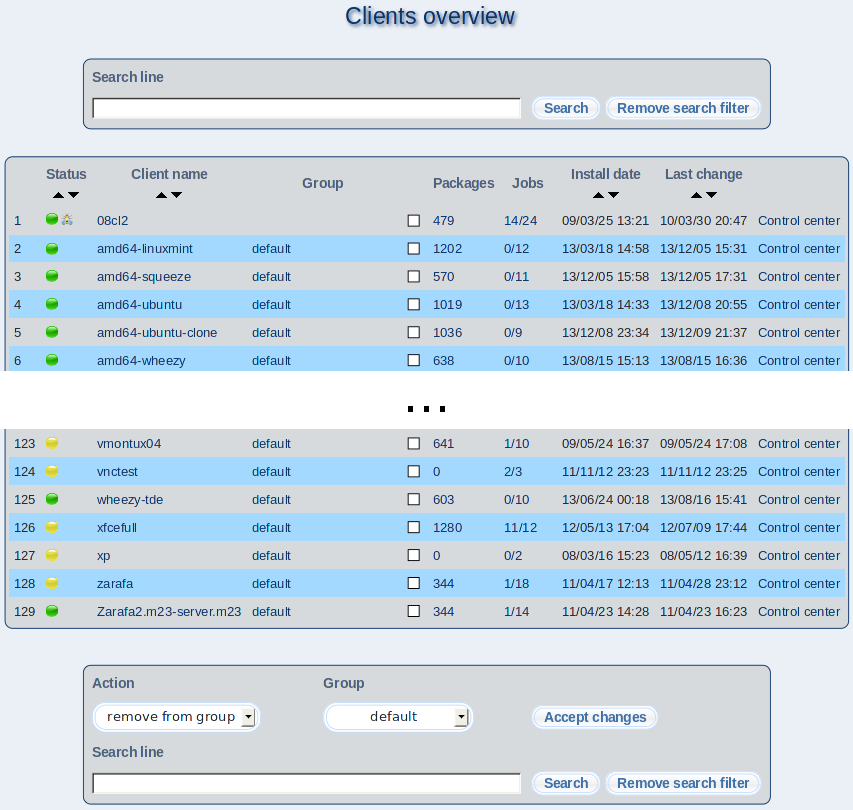
\includegraphics[scale=0.4]{/mdk/doc/manual/screenshots/de/clients_overview.png} \\
Klicken Sie auf den Clientnamen, erhalten Sie detaillierte Informationen zu dem gew�hlten Client und haben Zugriff auf das Kontrollzentrum.\\
\subsection{Statuserkl�rung}
Die Farbe des Statussymbols gibt an, wie weit die Installation des jeweiligen Clients vorangeschritten ist.\\
\begin{itemize}
\item \textbf{rot}: Client wurde aufgenommen, die automatische Hardwareerkennung ist nicht abgeschlossen.\\
\item \textbf{gelb}: Sie k�nnen den Client formatieren und partitionieren, das Basissystem wird automatisch zugewiesen.\\
\item \textbf{gr�n}: Das Basissystem des Clients ist eingerichtet, Sie k�nnen zus�tzliche Software installieren.\\
\item \textbf{blau}: Der Client installiert gerade zus�tzliche Software.\\
\item \textbf{orange}: Der Client ist im \textbf{kritischen Zustand}. D.h. bei der Installation ist ein Fehler aufgetreten, der vom Administrator behoben werden mu�. Im Kontrollzentrum gibt es eine Reihe von M�glichkeiten, den kritischen Zustand zu beheben.\\
\item \textbf{wei�}: Musterclient f�r die Masseninstallation, von dem die Einstellungen auf die anderen Clients �bertragen werden.\\
\item \textbf{Fliege (Bug)}: Zeigt an, da� sich ein Client im Debug-Modus befindet.\\
\end{itemize}
\subsection{Auftr�ge}
In dieser Spalte steht vor dem Schr�gstrich die Anzahl der noch nicht abgearbeiteten Auftr�ge und die Anzahl aller Auftr�ge dahinter.\\
\subsection{Mehrere Clients bearbeiten}
W�hlen Sie mehrere Clients dadurch aus, da� Sie den Haken in den Spalte mit den gew�nschten Clients setzen.\\
Danach k�nnen Sie verschiedene Aktionen mit allen gew�hlten Clients durchf�hren:\\
\begin{itemize}
	\item \textbf{Aus Gruppe l�schen}: W�hlen Sie hierzu die Gruppe aus, aus der die Clients gel�scht werden sollen. Sollte ein Client nicht in der angegebenen Gruppe sein, so wird mit diesem keine Aktion durchgef�hrt.\\
	\item \textbf{Zur Gruppe hinzuf�gen}: W�hlen Sie hierzu die Gruppe aus, zu der die Clients hinzugef�gt werden sollen. Ist ein Client bereits in dieser Gruppe vorhanden, so wird an seiner Gruppenzugeh�rigkeit nichts ge�ndert.\\
	\item \textbf{L�schen}: L�scht die gew�hlten Clients\\
\end{itemize}
\subsection{Hinweis}
Um den aktuellen Client-Status zu erhalten, benutzen Sie die Reload-Funktion Ihres Browsers (z.B. durch Dr�cken der Taste F5)\\
\subsection{Tricks}
\begin{itemize}
\item Durch Klicken auf das Statussysmbol kann der aktuelle Status des Clients ge�ndert werden.\\
\item Allerdings sollten Sie den Client-Status nur �ndern, wenn Sie wissen, was Sie tun. Der Debug-Modus kann durch einen Klick auf das Laus-Icon (de)aktiviert werden.\\
\end{itemize}
